We recall that our goal is to compute the expectation in \eqref{BS_formula_rbergomi}. In fact, as seen in Section \ref{sec:Simulation of the rBergomi model}, we need   $2N$-dimensional Gaussian inputs for the used  hybrid  scheme ($N$ is the number of time steps in  the time grid), namely
\begin{itemize}
	\item $\mathbf{W}^{(1)}=\{W^{(1)}_i\}_{i=1}^N$: The $N$ Gaussian random variables that are defined in Section  \ref{sec:The rBergomi model}.
	\item $\mathbf{W}^{(2)}=\{W^{(2)}_j\}_{j=1}^N$: An artificially introduced $N$ Gaussian random variables that are used for left-rule points in the hybrid scheme, as explained in Section  \ref{sec:Simulation of the rBergomi model}.
\end{itemize}
We can rewrite \eqref{BS_formula_rbergomi} as 
\begin{align}\label{BS_formula_rbergomi_2}
C_{\text{RB}}\left( T, K \right)&=\text{E}\left[C_{\text{BS}}\left( S_0 = \operatorname{exp}\left(\rho \int_0^T \sqrt{v_t} dW_t^1 - \frac{1}{2}
\rho^2 \int_0^T v_t dt\right),\ k = K, \ \sigma^2 = (1-\rho^2)
\int_0^T v_t dt \right) \right] \nonumber \\
&\approx \int_{\rset^{2N}} C_{BS} \left(G(\mathbf{w}^{(1)},\mathbf{w}^{(2)})\right) \rho_{N}(\mathbf{w}^{(1)})  \rho_{N}(\mathbf{w}^{(2)}) d\mathbf{w}^{(1)} d\mathbf{w}^{(2)} \nonumber \\
&:=C_{RB}^{N},
\end{align}
where $G$  maps  $2N$ independent standard Gaussian random inputs to the parameters fed to Black-Scholes formula, and  $\rho_N$ is the multivariate Gaussian density, given by 
\begin{equation*}\label{eq: multivariate gaussian distribution}
\rho_N(\mathbf{z})=\frac{1}{(2 \pi)^{N/2}} e^{-\frac{1}{2} \mathbf{z}^T \mathbf{z}} \PERIOD
\end{equation*} 
Therefore, the initial integration problem that we are solving lives in $2N$-dimensional space, which becomes very large as the number of time steps $N$, used in the hybrid scheme, increases.

Our approach of approximating the expectation in \eqref{BS_formula_rbergomi_2} is based on hierarchical deterministic quadratures, namely  i) ASGQ using the same construction in \cite{haji2016multi} and ii) randomized QMC based on lattice rules. We describe the ASGQ  method in our context in Section \ref{sec:Details of the MISC} and in Section \ref{sec:Quasi Monte Carlo (QMC)}, we provide details on the implented QMC method.  To make an effective use of either ASGQ or QMC methods, we  apply two techniques to overcome the issue of facing a high dimensional integrand due to the discretization scheme used for simulating the rBergomi dynamics. The first  consists of applying a hierarchical  path generation method, based on Brownian bridge (Bb) construction, with the aim of reducing the effective dimension as  described  in Section \ref{sec:Brwonian bridge construction}. The second technique consists of applying Richardson extrapolation to reduce the bias, resulting in reducing  the maximum number of dimensions needed for the integration problem. Details about  Richardson extrapolation  are provided in Section \ref{sec:Richardson extrapolation}.

If we denote by $\mathcal{E}_{\text{tot}}$ the total error of approximating the  expectation in \eqref{BS_formula_rbergomi} using the ASGQ estimator, $Q_N$, then we have a natural error decomposition
\begin{align}\label{eq:total_error_ASGQ}
\mathcal{E}_{\text{tot}} & \le \abs{C_{\text{RB}}-C_{\text{RB}}^N}+\abs{C_{\text{RB}}^N-Q_{N}} \le \mathcal{E}_B(N)+ \mathcal{E}_Q(\text{TOL}_{\text{ASGQ}},N),
\end{align}
where  $\mathcal{E}_Q$ is the quadrature error, $\mathcal{E}_B$  is the bias, $\text{TOL}_{\text{ASGQ}}$ is a user selected tolerance for ASGQ method, and $C_{\text{RB}}^N$ is the biased price computed with $N$ time steps as given by \eqref{BS_formula_rbergomi_2}.

On the other hand, the total error of approximating the  expectation in \eqref{BS_formula_rbergomi} using the randomized QMC or MC estimator, $Q^{\text{MC(QMC)}}_N$ can be bounded by

\begin{align}\label{eq:total_error_MC}
	\mathcal{E}_{\text{tot}} & \le \abs{C_{\text{RB}}-C_{\text{RB}}^N}+\abs{C_{\text{RB}}^N-Q^{\text{MC (QMC)}}_N} \le \mathcal{E}_B(N)+ \mathcal{E}_{S}(M,N),
\end{align}
where  $\mathcal{E}_S$ is the statistical error\footnote{The statistical error estimate of MC or randomized QMC is  $C_{\alpha} \frac{\sigma_M}{\sqrt{M}}$, where $M$ is the number of samples and $C_{\alpha}=1.96$ for $95\%$ confidence interval.}, $M$ is the number of samples used for MC or randomized QMC method.
\subsection{Adaptive sparse grids quadrature (ASGQ)}\label{sec:Details of the MISC}

We assume that we want to approximate the expected value $\text{E}[f(Y)]$ of an analytic function $f\colon \Gamma \to \rset$ using a tensorization of quadrature formulas over $\Gamma$.

To introduce simplified notations, we start with the one-dimensional case. Let us denote by $\beta$ a non-negative integer, referred to as a ``stochastic discretization level", and by $m: \nset \rightarrow \nset$  a strictly increasing function with $m(0)=0$ and $m(1)=1$, that we call  ``level-to-nodes function". At level $\beta$, we consider a set of $m(\beta)$ distinct quadrature points in $\rset$, $\mathcal{H}^{m(\beta)}=\{y^1_\beta,y^2_\beta,\dots,y_\beta^{m(\beta)}\} \subset \rset$, and a set of quadrature weights, $\boldsymbol{\omega}^{m(\beta)}=\{\omega^1_\beta,\omega^2_\beta,\dots,\omega_\beta^{m(\beta)}\}$. We also let $C^0(\rset)$ be the set of real-valued continuous functions over $\rset$. We then define the quadrature operator as
\begin{equation*}
Q^{m(\beta)}:C^0(\rset) \rightarrow \rset, \quad Q^{m(\beta)}[f]= \sum_{j=1}^{m(\beta)} f(y^j_\beta) \omega_\beta^j.
\end{equation*}
In our case, we have in \eqref{BS_formula_rbergomi_2} a multi-variate integration problem with,  $f=C_{\text{BS}}\circ G$, $\mathbf{Y}=(\mathbf{W}^{(1)},\mathbf{W}^{(2)})$, and  $\Gamma=\rset^{2N}$, in the previous notations. Furthermore, since we are dealing with Gaussian densities, using Gauss-Hermite quadrature points is the appropriate choice.

We define for any multi-index $\boldsymbol{\beta} \in \nset^{2N}$
$$Q^{m(\boldsymbol{\beta})}: C^0(\rset^{2N}) \rightarrow \rset,\quad  Q^{m(\boldsymbol{\beta})}= \bigotimes_{n = 1}^{2N} Q^{m(\beta_n)} \COMMA $$
where the $n$-th quadrature operator is understood to act only on the $n$-th variable of $f$. Practically, we obtain the value of $Q^{m(\boldsymbol{\beta})}[f]$  by using the grid $\mathcal{T}^{m(\boldsymbol{\beta})}= \prod_{n = 1}^{2N}  \mathcal{H}^{m(\beta_n)}$, with cardinality $\#\mathcal{T}^{m(\boldsymbol{\beta})}=\prod_{n=1}^{2N} m (\beta_n)$, and computing
$$ Q^{m(\boldsymbol{\beta})}[f]= \sum_{j=1}^{\#\mathcal{T}^{m(\boldsymbol{\beta})}} f(\hat{y}_j) \bar{\omega}_j \COMMA$$
where $\hat{y}_j \in \mathcal{T}^{m(\boldsymbol{\beta})}$ and $\bar{\omega}_j$ are  products of weights of the univariate quadrature rules. To simplify notation, hereafter, we replace  $Q^{m(\boldsymbol{\beta})}$ by $Q^{\boldsymbol{\beta}}$.

A direct approximation $\expt{f[\mathbf{Y}]} \approx Q^{\boldsymbol{\beta}}[f]$ is not an appropriate option  due to the well-known ``curse of dimensionality". We use  a hierarchical ASGQ\footnote{More details about sparse grids can be found in \cite{bungartz2004sparse}.} strategy, specifically using the same
construction as in \cite{haji2016multi}, and which uses  stochastic discretizations  and a classic sparsification approach to obtain an effective approximation scheme for $\expt{f}$. 

To be concrete, in our setting, we are left with a $2N$-dimensional Gaussian random input, which is chosen independently, resulting in  $2N$ numerical parameters for ASGQ, which we use as the basis of the multi-index construction. For a multi-index $\boldsymbol{\beta} = (\beta_n)_{n=1}^{2N} \in \mathbb{N}^{2N}$, we denote  by
$Q_N^{\boldsymbol{\beta}}$,   the result of approximating \eqref{BS_formula_rbergomi_2} with a number of quadrature points  in the $i$-th dimension equal to  $m(\beta_i)$. We further define the set of
differences $\Delta Q_N^{\boldsymbol{\beta}}$ as follows: for a single index $1 \le i \le 2N$,
let
\begin{equation*}
\Delta_i Q_N^{\boldsymbol{\beta}} = \left\{ 
\aligned 
 Q_N^{\boldsymbol{\beta}} &- Q_N^{\boldsymbol{\beta}'}  \text{, with } \boldsymbol{\beta}' =\boldsymbol{\beta} - e_i, \text{ if } \boldsymbol{\beta}_i>0 \COMMA \\
 Q_N^{\boldsymbol{\beta}} &, \quad  \text{ otherwise,}
\endaligned
\right.
\end{equation*}
where $e_i$ denotes the $i$th $2N$-dimensional unit vector. Then, $\Delta
Q_N^{\boldsymbol{\beta}}$ is defined as
\begin{equation*}
\Delta Q_N^{\boldsymbol{\beta}} = \left( \prod_{i=1}^{2N} \Delta_i \right) Q_N^{\boldsymbol{\beta}}.
\end{equation*}
For instance, when $N = 1$, then 
\begin{multline*}
	\Delta Q_1^{\boldsymbol{\beta}} = \Delta_2 \Delta_1 Q_1^{(\beta_1, \beta_2)} = \Delta_2\left( Q_1^{(\beta_1,
		\beta_2)} - Q_1^{(\beta_1-1,\beta_2)} \right) = \Delta_2 Q_1^{(\beta_1,
		\beta_2)} - \Delta_2 Q_1^{(\beta_1-1,\beta_2)} 
	\\= Q_1^{(\beta_1, \beta_2)} - Q_1^{(\beta_1, \beta_2-1)} - Q_1^{(\beta_1-1, \beta_2)} + Q_1^{(\beta_1-1, \beta_2-1)}.
\end{multline*}
Given the definition of $C_{RB}^{N}$ by \eqref{BS_formula_rbergomi_2}, we have the telescoping property
\begin{equation*}
C_{RB}^{N}=Q_N^\infty = \sum_{\beta_1=0}^\infty \cdots \sum_{\beta_{2N} = 0}^\infty \Delta
Q_N^{(\beta_1, \ldots, \beta_{2N})} = \sum_{\boldsymbol{\beta} \in \mathbb{N}^{2N}} \Delta Q_N^{\boldsymbol{\beta}}.
\end{equation*}
The ASGQ estimator used for approximating \eqref{BS_formula_rbergomi_2}, and using a set of multi-indices $\mathcal{I}\subset \nset^{2N}$ is given by
\begin{equation}\label{eq:MISC_quad_estimator}
	Q_N^{\mathcal{I}} = \sum_{\boldsymbol{\beta} \in \mathcal{I}} \Delta Q_N^{\boldsymbol{\beta}}.
\end{equation}
The quadrature error in this  case  is given by
\begin{equation}\label{eq:quadrature error}
	\mathcal{E}_Q(\text{TOL}_{\text{ASGQ}},N) =\abs{Q_N^\infty - Q_N^\mathcal{I}} \le \sum_{\boldsymbol{\beta} \in \mathbb{N}^{2N} \setminus
		\mathcal{I}} \abs{\Delta Q_N^{\boldsymbol{\beta}}}.
\end{equation}
We define the work contribution, $\Delta \mathcal{W}_{\boldsymbol{\beta}}$, to be the computational cost  required to add  $\Delta Q_N^{\boldsymbol{\beta}}$ to $Q^{\mathcal{I}}_N$, and the error contribution, $\Delta E_{\boldsymbol{\beta}}$, to be  a measure of how much the quadrature error, defined in \eqref{eq:quadrature error}, would decrease once $\Delta Q_N^{\boldsymbol{\beta}}$  has been added to  $Q^{\mathcal{I}}_N$, that is 
\begin{align}\label{eq:Work_error_contributions}
\Delta E_{\boldsymbol{\beta}} &= \abs{Q^{\mathcal{I} \cup \{\boldsymbol{\beta}\}}_N-Q^{\mathcal{I}}_N}\\
\Delta \mathcal{W}_{\boldsymbol{\beta}} &= \text{Work}[Q^{\mathcal{I} \cup \{\boldsymbol{\beta}\}}_N]-\text{Work}[Q^{\mathcal{I}}_N].
\end{align}
 The  construction of the optimal  $\mathcal{I}$ is done by profit thresholding (see Figure \ref{fig:Construction of the index set for ASGQ method} for illustration), that is, for a certain threshold value $\bar{T}$, and a profit of a hierarchical surplus defined by
 \begin{equation*}
 P_{\boldsymbol{\beta}}= \frac{\abs{\Delta E_{\boldsymbol{\beta}}}}{\Delta\mathcal{W}_{\boldsymbol{\beta}}},
 \end{equation*}
the optimal index set  $\mathcal{I}$  for our ASGQ is given by 
 $\mathcal{I}=\{\boldsymbol{\beta}: P_{\boldsymbol{\beta}}	 \ge \bar{T}\}$. 
 \FloatBarrier
 \begin{figure}[htb]
 	\centering % <-- added
 	\begin{subfigure}{0.165\textwidth}
 		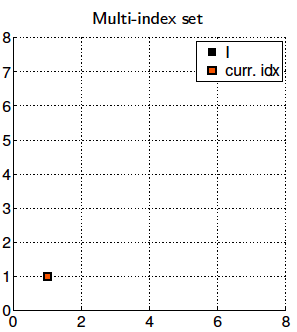
\includegraphics[width=\linewidth]{./figures/MISC_construction/1}
 		\caption{}
 		\label{fig:1}
 	\end{subfigure}\hfil % <-- added
 	\begin{subfigure}{0.165\textwidth}
 		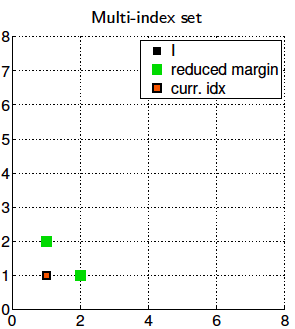
\includegraphics[width=\linewidth]{./figures/MISC_construction/2}
 		\caption{}
 		\label{fig:2}
 	\end{subfigure}\hfil % <-- added
 	\begin{subfigure}{0.165\textwidth}
 		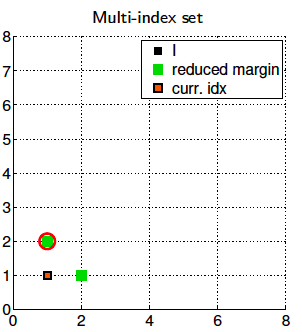
\includegraphics[width=\linewidth]{./figures/MISC_construction/3}
 		\caption{}
 		\label{fig:3}
 	\end{subfigure}
 	\medskip
 	\begin{subfigure}{0.165\textwidth}
 		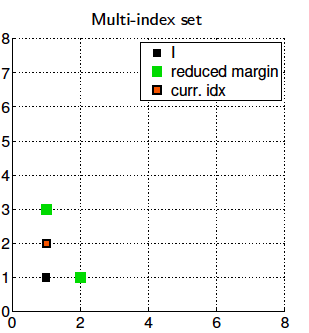
\includegraphics[width=\linewidth]{./figures/MISC_construction/4}
 		\caption{}
 		\label{fig:4}
 	\end{subfigure}\hfil % <-- added
 	\begin{subfigure}{0.165\textwidth}
 		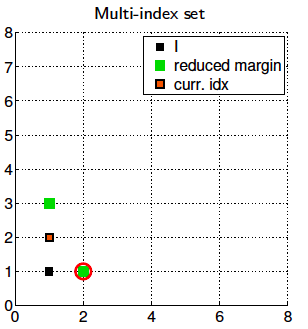
\includegraphics[width=\linewidth]{./figures/MISC_construction/5}
 		\caption{}
 		\label{fig:5}
 	\end{subfigure}\hfil % <-- added
 	\begin{subfigure}{0.165\textwidth}
 		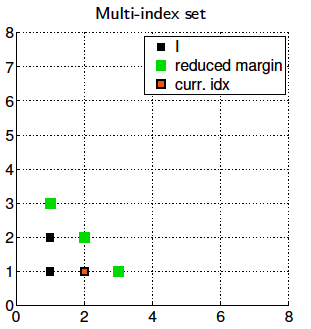
\includegraphics[width=\linewidth]{./figures/MISC_construction/6}
 		\caption{}
 		\label{fig:6}
 	\end{subfigure}
 	\caption{Construction of the index set for ASGQ method. A posteriori, adaptive construction: Given an index set $\mathcal{I}_k$, compute the profits of the neighbor indices and select the most profitable one.}
 	\label{fig:Construction of the index set for ASGQ method}
 \end{figure}
\FloatBarrier

\begin{remark}
	The choice of the hierarchy of quadrature points, $m(\boldsymbol{\beta})$, is flexible in the ASGQ algorithm and can be fixed by the user, depending on the convergence properties of the problem at hand. For instance, for the sake of reproducibility, in our numerical experiments we used a linear hierarchy: $m(\beta)=4 (\beta-1)+1,\: 1 \le \beta $, for results of parameter set $1$ in Table \ref{table:Reference solution, using MC with $500$ time steps, of Call option price under rBergomi model, for different parameter constellation.}. For the remaining parameter sets in Table  \ref{table:Reference solution, using MC with $500$ time steps, of Call option price under rBergomi model, for different parameter constellation.}, we used a geometric hierarchy: $m(\beta)=2^{\beta-1}+1, \:1 \le \beta $.
\end{remark} 
\begin{remark}
As emphasized in \cite{haji2016multi}, one important requirement to get the optimal performance of the ASGQ is to check  the error convergence, defined by \eqref{eq:Work_error_contributions},  of first and mixed difference operators. We checked this requirement in all our numerical experiments, and for illustration, we show in Figures  \ref{fig:first_diff_comp_K_1_H_002} and \ref{fig:second_diff_comp_K_1_H_002}, the error convergence of first and second order differences for the case of parameter set $2$ in Table \ref{table:Reference solution, using MC with $500$ time steps, of Call option price under rBergomi model, for different parameter constellation.}.  These plots show that: i) $\Delta \text{E}_{\boldsymbol{\beta}}$ decreases exponentially fast with respect to $\beta_i$, and ii) $\Delta \text{E}_{\boldsymbol{\beta}}$ has a  product structure since  we  observe  a faster error decay for second differences compared to corresponding first difference operators.
\end{remark} 

\begin{figure}[h!]
	\centering
	\begin{subfigure}{.4\textwidth}
		\centering
		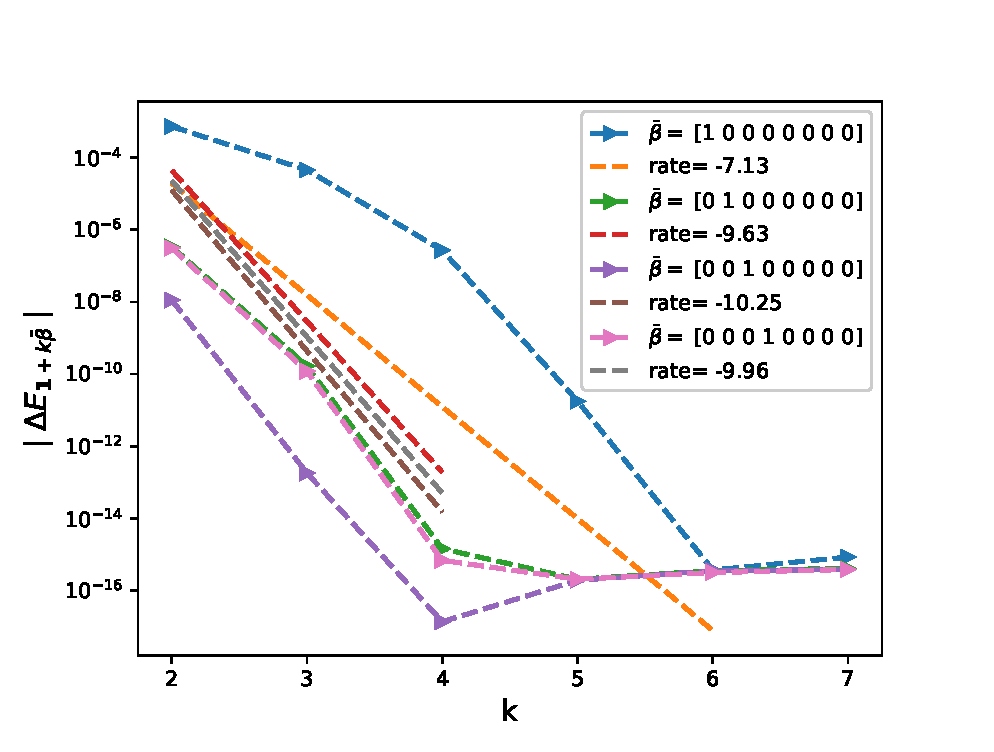
\includegraphics[width=1\linewidth]{./figures/rBergomi_mixed_error_rates/without_change_measure/N_4/H_002/first_difference_rbergomi_4steps_H_002_K_1_totally_hierarch_with_rate_W1}
		\caption{}
		\label{fig:sub3}
	\end{subfigure}%
	\begin{subfigure}{.4\textwidth}
		\centering
		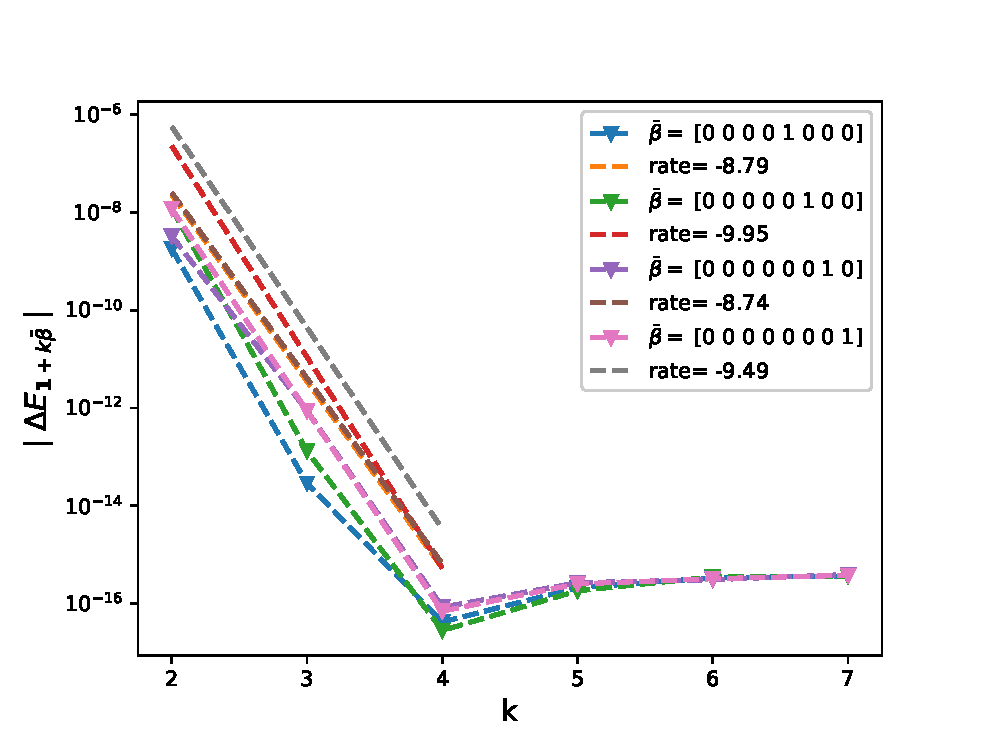
\includegraphics[width=1\linewidth]{./figures/rBergomi_mixed_error_rates/without_change_measure/N_4/H_002/first_difference_rbergomi_4steps_H_002_K_1_totally_hierarch_with_rate_W2}
		\caption{}
		\label{fig:sub4}
	\end{subfigure}
	
	
	
	\caption{The rate of error convergence of first order differences $\abs{\Delta \text{E}_{\boldsymbol{\beta}}}$, defined by \eqref{eq:Work_error_contributions}, ($\boldsymbol{\beta}=\mathbf{1}+k \bar{\boldsymbol{\beta}}$) with respect to $\mathbf{W}^{(1)}$ (a)  and  with respect to $\mathbf{W}^{(2)}$ (b), for parameter set $2$ in Table \ref{table:Reference solution, using MC with $500$ time steps, of Call option price under rBergomi model, for different parameter constellation.}. The number of quadrature points used in the $i$-th dimension is $N_i=2^{\beta_i-1}+1$. }
	\label{fig:first_diff_comp_K_1_H_002}
\end{figure}


\begin{figure}[h!]
	\centering
	\begin{subfigure}{.4\textwidth}
		\centering
		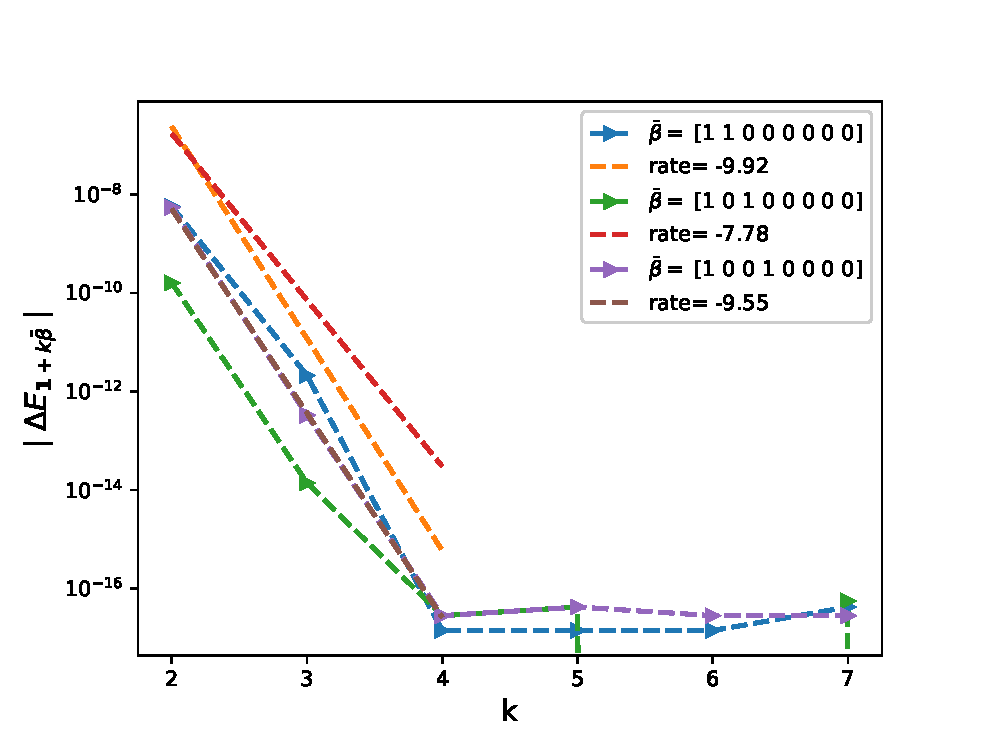
\includegraphics[width=1\linewidth]{./figures/rBergomi_mixed_error_rates/without_change_measure/N_4/H_002/mixed_difference_order2_rbergomi_4steps_H_002_K_1_totally_hierarch_with_rate_W1}
		\caption{}
		\label{fig:sub3}
	\end{subfigure}%
	\begin{subfigure}{.4\textwidth}
		\centering
		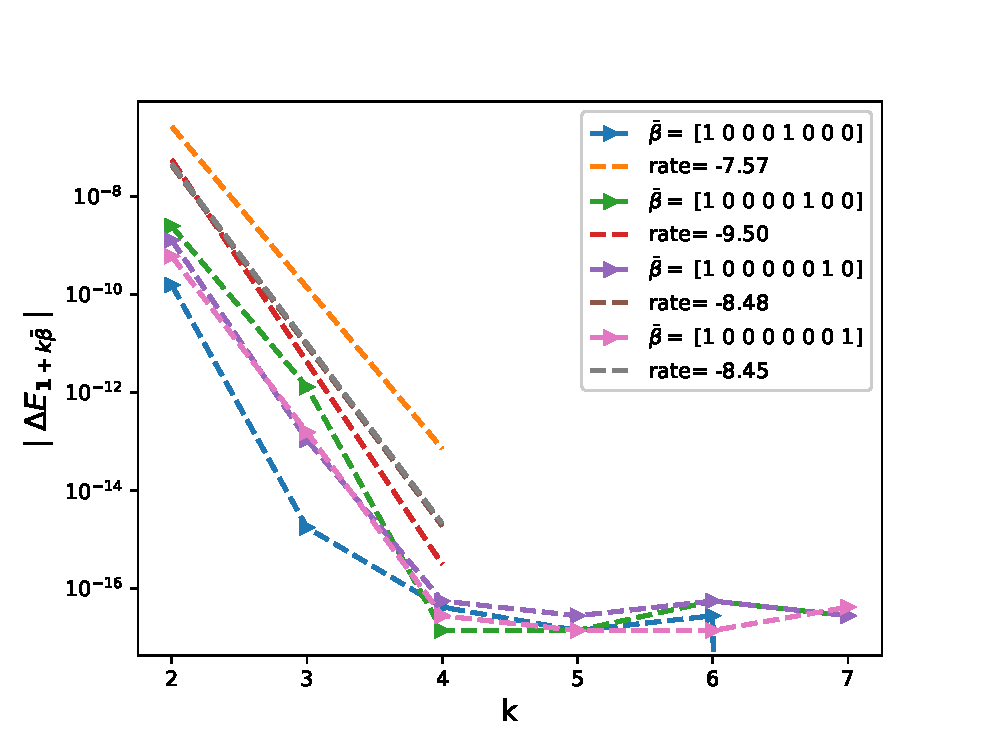
\includegraphics[width=1\linewidth]{./figures/rBergomi_mixed_error_rates/without_change_measure/N_4/H_002/mixed_difference_order2_rbergomi_4steps_H_002_K_1_totally_hierarch_with_rate_W2}
		\caption{}
		\label{fig:sub4}
	\end{subfigure}
	
	\caption{The rate of error convergence of  second order differences $\abs{\Delta \text{E}_{\boldsymbol{\beta}}}$, defined by \eqref{eq:Work_error_contributions},  ($\boldsymbol{\beta}=\mathbf{1}+k \bar{\boldsymbol{\beta}}$) with respect to $\mathbf{W}^{(1)}$ (a)  and  with respect to $\mathbf{W}^{(2)}$ (b), for parameter set $2$ in Table \ref{table:Reference solution, using MC with $500$ time steps, of Call option price under rBergomi model, for different parameter constellation.}. The number of quadrature points used in the $i$-th dimension is $N_i=2^{\beta_i-1}+1$.}
	\label{fig:second_diff_comp_K_1_H_002}
\end{figure}

\FloatBarrier

\begin{remark}
The analiticity assumption, stated in the beginning of Section \ref{sec:Details of the MISC}, is crucial for the optimal performance of our proposed method. In fact, although we face the issue of the  ``curse of dimensionality" when increasing $N$, the analiticity of $f$ implies a spectral convergence for sparse grids quadrature.
\end{remark} 
%
%\begin{remark}
%	In this paper, we limited ourselves to designing a novel alternative method  based on hierarchical adaptive sparse grids quadrature for computing option prices under the rBergomi model. Giving the significant performance gains of our novel designed algorithm, we expect that designing a method based on QMC can bring similar or more gains as  our approach.
%\end{remark}


%\red{\subsubsection{ASGQ error estimate}
%As discussed, potential ways of estimating the quadrature error are presented below.
\subsection{First way: Similar to the one implemented by Joakim}
I think this way is almost similar to the one implemented by Joakim. He may correct me if I missed some things.

In our case, once we fix $N$, we define from \eqref{BS_formula_rbergomi_2}
\begin{equation*}
F^N=C_{\text{BS}}(G(\mathbf{W}^{(1)},\mathbf{W}^{(2)})) \PERIOD
\end{equation*}
We introduce the set $C^0(\rset)$ of real-valued continuous functions over $\rset$, and the subspace of polynomials of degree at most $q$ over $\rset$, $\mathbb{P}^q(\rset) \subset C^0(\rset)$. Next,
we consider a sequence of univariate Lagrangian interpolant operators in each dimension $Y_n$ ($1 \le n \le 2N$), that is, $\{U_n^{m(\beta_n)}\}_{\beta_n \in \nset_+}$ (we refer to the value $\beta_n$ as the interpolation level). Each interpolant is built over a set of $m(\beta_n)$ collocation points, $\mathcal{H}^{m(\beta_n)}=\{y^1_n,y^2_n,\dots,y^{m(\beta_n)}_n\} \subset \rset$, thus, the interpolant yields a polynomial approximation,
\begin{equation*}
U^{m(\beta_n)}:C^0(\rset) \rightarrow \mathbb{P}^{m(\beta_n)-1}(\rset), \quad U^{m(\beta_n)}[F^N](y_n)= \sum_{j=1}^{m(\beta_n)} \left( f(y^j_n) \prod_{k=1;k \neq j}^{m(\beta_n)} \frac{y_n-y_n^k}{y_n^j-y_n^k}\right) \PERIOD
\end{equation*}
The $2N$-variate Lagrangian interpolant can then be built by a tensorization of univariate interpolants: denote by $C^0(\rset^{2N})$ the space of real-valued $2N$-variate continuous functions over $\rset^{2N}$ and by $\mathbb{P}^{\mathbf{q}}(\rset^{2N}) = \otimes_{n=1}^{2N} \mathbb{P}^{\mathbf{q}_n}(\rset)$ the subspace of polynomials of degree at most $q_n$ over $\rset$, with $\mathbf{q}=(q_1,\dots,q_{2N})\in  \nset^{2N}$, and consider a multi-index $\boldsymbol{\beta} \in \nset^{2N}_+$ assigning the interpolation level in each direction, $y_n$, then  the multivariate interpolant can then be written as
$$U^{m(\boldsymbol{\beta})}: C^0(\rset^{2N}) \rightarrow \mathbb{P}^{m(\boldsymbol{\beta})-1}(\rset^{2N}) ,\quad  U^{m(\boldsymbol{\beta})}[F^N](\mathbf{y})= \bigotimes_{n = 1}^{2N} U^{m(\beta_n)} [F^N](\mathbf{y}) \PERIOD $$
Given this construction, we can define the ASGQ interpolant  for approximating $F^N$, using a set of multi indices $\mathcal{I} \in \nset^{2N}$ as
\begin{equation}
I^{\mathcal{I}}[F^N]= \sum_{\boldsymbol{\beta} \in \mathcal{I}} \Delta U_N^{\boldsymbol{\beta}} \COMMA
\end{equation}
where 
\begin{equation*}
\Delta_i U_N^{\boldsymbol{\beta}} = \left\{ 
\aligned 
 U_N^{\boldsymbol{\beta}} &- U_N^{\boldsymbol{\beta}'}  \text{, with } \boldsymbol{\beta}' =\boldsymbol{\beta} - e_i, \text{ if } \boldsymbol{\beta}_i>0 \\
 U_N^{\boldsymbol{\beta}} &, \quad  \text{ otherwise,}
\endaligned
\right.
\end{equation*}
where $e_i$ denotes the $i$th $2N$-dimensional unit vector. Then, $\Delta
U_N^{\boldsymbol{\beta}}$ is defined as
\begin{equation*}
\Delta U_N^{\boldsymbol{\beta}} = \left( \prod_{i=1}^{2N} \Delta_i \right) U_N^{\boldsymbol{\beta}}.
\end{equation*}
We define the interpolation error induced by ASGQ as
\begin{equation}
e_{N}= F^N-I^{\mathcal{I}}[F^N] \PERIOD
\end{equation}
One can have a bound on the interpolation error of ASGQ, $e_{N}$, by tensorizing one dimensional error estimates, and  then simply integrate that bound to get the ASGQ  error, $\mathcal{E}_Q(\text{TOL}_{\text{ASGQ}},N)$, defined in \eqref{eq:total_error_ASGQ}. However, we think that this will  not lead to a sharp error estimate for ASGQ. Another strategy for estimating the ASGQ  error, is to estimate $\expt{e_N}$ using MC by sampling directly $e_N$ (what I think Jaokim code is doing actually) .

If we define $Y=F^N+(Q_N^{\mathcal{I}}-I^{\mathcal{I}}[F^N])$ (where $Q_N^{\mathcal{I}}$ is the ASGQ  estimator), then we have
\begin{align}\label{eq:Control_variate}
\expt{Y}&=\expt{F^N}\nonumber\\
Var[Y]&=Var[e_N]< Var[\mathcal{A}_{\text{MC}}]\COMMA
\end{align}
where $\mathcal{A}_{\text{MC}}$ is the MC estimator for $\expt{F^N}$.

\eqref{eq:Control_variate} shows that ASGQ can be seen as a control variate for MC estimator and consequently as a powerful variance reduction tool.

This way of estimating the quadrature error comes with the disadvantage of exciting the strong error which has a poor behavior in our context resulting maybe to having a non-sharp error estimate. In fact, by the central limit theorem, we expect that
\begin{align}\label{eq:CLT_interpol_errror}
\abs{\expt{e_N}}&=\abs{\int \underbrace{F^N-I^{\mathcal{I}}[F^N](y)}_{Y(y)} dy}\nonumber\\
&\approx \frac{C_\alpha}{\sqrt{M}} \sqrt{\text{Var(Y)}}\PERIOD
\end{align}
In our context of the rBergomi model we know that the strong error is of order $H$, that is we expect to have $\text{Var(Y)}=\Ordo{h^H}$ ($h$ is the mesh size and $H$ is the Hurst parameter which is of order $\approx 0.1$. As a consequence, it may be that using this way will not provide a sharp enough error estimate for the quadrature error!

\subsection{Second way}
To avoid exciting the strong error when estimating the quadrature error and just act on the weak error, we can use a second way that is inspired of randomized QMC. In fact, we suggest to use a randomized version of ASGQ where the randomization involves randomized rotation and scaling for quadrature rules since we deal with unbounded domains and Hermite quadrature rule. Although this comes with the advantage of just acting on the weak error, it has the issue of reducing anisotropy which is a main feature for a good performance of ASGQ.

We can formulate this more in case the first way fail!

\subsection{Third way}
One can learn the error curve as a way to reduce the extra burden that comes
from estimating the ASGQ error but this not yet formulated yet. I will try to formulate it if the two previous options fail!
%}

\subsection{Quasi Monte Carlo (QMC)}\label{sec:Quasi Monte Carlo (QMC)}
\red{A second type of deterministic quadrature that we test in this work is the QMC method. Specifically, we use the lattice rules family of QMC \cite{sloan1985lattice,cools2008belgian,nuyens2014construction}.  The main input for the lattice rule is one integer vector with $d$ component ($d$ dimension of the integration problem).

In fact, given an integer vector $z = (z_1,\dots, z_d)$ known as \textit{the generating vector}, a (rank-$1$) lattice rule with $n$ points takes the form

\begin{equation}
Q_n(f):=\frac{1}{n}\sum_{k=0}^{n-1} f \left( \frac{kz \: \text{mod}\: n}{n}\right).
\end{equation}
The quality of the lattice rule depends on the choice of the generating vector. Due to the modulo operation, it suffices to consider the values from $1$ up to $n-1$, leaving out $0$ which is clearly a bad choice. Furthermore, we restrict the values to those relatively prime to $n$, to ensure that every one-dimensional projection of the $n$ points yields $n$ distinct values. Thus, we write $\mathbf{z} \in \mathbb{U}_n^d$, with $\mathbb{U}_n:=\{z \in \zset: 1 \le z \le n-1\: \text{and gcd}(z,n)=1\}$. For practical purposes,  we choose $n$  to be a power of $2$. The total number of possible choices for the generating vector is then  $(n/2)^d$. 

To get an unbiased approximation of the integral, we use  a randomly shifted lattice rule, which also allows us to obtain a practical error estimate in the same way as the MC method. It works as follows. We generate $q$ independent random shifts $\Delta^{(i)}$ for $i=0,\dots,q-1$ from the uniform distribution on $[0,1]^d$ . For the same fixed lattice generating vector $z$, we compute the $q$ different shifted lattice rule approximations and denote
them by $Q^{(i )}_n(f)$ for $i=0,\dots,q-1$.We then take the average
\begin{align}
\overline{Q}_{n,q}(f)=\frac{1}{q} \sum_{i=0}^{q-1}Q^{(i )}_n(f)=\frac{1}{q}\sum_{i=0}^{q-1}\left(\frac{1}{n}\sum_{k=0}^{n-1} f \left( \frac{kz+\Delta^{(i)}  \: \text{mod}\: n}{n}\right)  \right)
\end{align}
as our final approximation to the integral.

We note that since we are dealing with Gaussian randomness and with integrals in infinite support, we use the inverse of the standard normal cumulative distribution function as a pre-transformation to map the problem to $[0,1]$ and then use QMC. Furthermore, in our numerical test, we use a pre-made point generators using latticeseq\_b2.py in python from   \url{https://people.cs.kuleuven.be/~dirk.nuyens/qmc-generators/}.
}

\subsection{Brownian bridge (Bb) construction}\label{sec:Brwonian bridge construction}
In the literature of ASGQ and  QMC, several hierarchical path generation methods (PGMs) have been proposed to reduce the effective dimension. Among these techniques, we mention  the Bb  construction \cite{morokoff1994quasi,moskowitz1996smoothness,caflisch1997valuation}, the principal component analysis (PCA)  \cite{acworth1998comparison} and the linear transformation (LT) \cite{imai2004minimizing}.

In our context, the Brownian motion on a time discretization  can be constructed either sequentially using a standard random walk construction, or hierarchically using   other PGMs as listed above. For our purposes, to make an effective use of ASGQ or QMC methods, which benefit from anisotropy, we use the Bb construction since it produces  dimensions with different importance, contrary to a random walk procedure for which all the dimensions of the stochastic space have equal importance. In fact, Bb uses the first several coordinates of the low-discrepancy points to determine the general shape of the Brownian path, and the last few coordinates influence only the fine detail of the path. Consequently, this representation  reduces the effective dimension  of the problem, which results in accelerating the ASGQ and QMC methods by reducing the computational cost.

Let us denote $\{t_i\}_{i=0}^{N}$ the grid of time steps. Then the Bb construction \cite{glasserman2004monte} consists of the following: given a past value $B_{t_i}$ and a future value $B_{t_k}$, the value $B_{t_j}$ (with $t_i < t_j < t_k$) can be generated according to 
\begin{equation*}
B_{t_j}=(1-\rho) B_{t_i}+\rho B_{t_k}+ \sqrt{\rho (1-\rho)(k-i) \Delta t} z, \: z \sim \mathcal{N}(0,1) \COMMA
\end{equation*}
where $\rho=\frac{j-i}{k-i}$.  

\subsection{Richardson extrapolation}\label{sec:Richardson extrapolation}
Another representation that we couple with the ASGQ and QMC methods is Richardson extrapolation \cite{talay1990expansion}. In fact, applying level $K_\text{R}$ (level of extrapolation) of Richardson extrapolation  dramatically reduces the bias, and as a consequence reduces the  number of time steps $N$ needed in the coarsest level to achieve a certain error tolerance. As a consequence, Richardson extrapolation directly reduces  the total dimension of the integration problem for achieving some error tolerance.

Let us denote by $(X_t)_{0 \le t \le T}$ a certain stochastic process and by $(\hat{X}_{t_i}^h)_{0 \le  t_i \le T}$ its approximation using a suitable  scheme with a time step $h$.  Then, for sufficiently small $h$, and a suitable smooth function $f$, we assume that
\begin{align}\label{Euler_weak_error_strenghten}
	\expt{f(\hat{X}_T^h)}= \expt{f(X_T)} + c h +\Ordo{h^2} \PERIOD
\end{align}
Applying \eqref{Euler_weak_error_strenghten} with discretization step $2h$, we  obtain
\begin{align*}
	\expt{f(\hat{X}_T^{2h})}= \expt{f(X_T)} + 2 c h +\Ordo{h^2} \COMMA
\end{align*}
implying
\begin{align*}
	2 \expt{f(\hat{X}_T^{2h})}- \expt{f(\hat{X}_T^{h})} =\expt{f(X_T)} + \Ordo{h^2} \PERIOD
\end{align*}
For higher levels of extrapolations, we use the following: Let us denote by $h_J=h_0 2^{-J}$ the grid sizes (where $h_0$ is the coarsest grid size), by $K_\text{R}$ the level of the Richardson extrapolation, and by $I(J,K_\text{R})$ the approximation of $\expt{f(X_T)}$ by terms up to level $K_\text{R}$ (leading to a weak error of order $K_\text{R}$), then we have the following recursion 
\begin{align*}
I(J,K_\text{R})=\frac{2^{K_\text{R}}I(J,K_\text{R}-1)-I(J-1,K_\text{R}-1)}{2^{K_\text{R}}-1},\quad J=1,2,\dots, K_\text{R}=1,2,\dots
\end{align*}
\begin{remark}
We emphasize that throughout our work, we are interested in the pre-asymptotic regime (a small number of time steps), and the use of Richardson extrapolation is justified by conjecture \ref{conj: Weak error structure} and our observed experimental results in that regime (see Section \ref{sec:Weak error plots_no_change}),  which suggest  a convergence of order one for the weak error. 
\end{remark}

%
%Although, we do not claim that the observed rates will scale well in the asymptotic regime, we did observe that the pre-asymptotic regime is enough to get sufficiently accurate estimates for the option prices. Furthermore, we emphasize that no proper weak error analysis has been done in the rough volatility context. 
